\chapter{TỔNG QUAN}
\label{chap:tongquan}

\section{Lý do chọn đề tài}

Hệ điều hành Microsoft Windows hiện chiếm hơn 75\% thị phần máy trạm trên toàn cầu và là mục tiêu trọng điểm của phần lớn các chiến dịch tấn công mạng nâng cao, từ các mối đe dọa tấn công có chủ đích kéo dài (Advanced Persistent Threat - APT), mã độc tống tiền (ransomware) cho đến các kỹ thuật tấn công không dùng tệp (fileless) và lạm dụng các công cụ hệ thống hợp quy. Trước sự tinh vi ngày càng tăng của kẻ tấn công, các giải pháp bảo vệ thiết bị đầu cuối truyền thống dựa trên chữ ký tĩnh và các chỉ số xâm nhập đã bộc lộ nhiều hạn chế: chúng gần như bị vô hiệu hóa trước các cuộc tấn công zero-day, các kỹ thuật không dùng tệp hay các biến thể mã độc mới chưa từng xuất hiện. Do đó, bảo mật hiện đại đang dịch chuyển mạnh mẽ sang hướng giám sát hành vi theo thời gian thực trên các thiết bị đầu cuối thông qua các hệ thống phát hiện và phản ứng tại điểm cuối (Endpoint Detection and Response - EDR).

Nhiều nghiên cứu đã chứng minh tính hiệu quả của hướng tiếp cận dựa trên hành vi và đồ thị nhân quả nguồn gốc trong việc phát hiện các cuộc tấn công nâng cao mà không cần định nghĩa trước mẫu tấn công, tiêu biểu là UNICORN \cite{han2020unicorn} và ATLAS \cite{alsaheel2021atlas}. Bên cạnh đó, các hạ tầng giám sát kernel-level như Event Tracing for Windows và Sysmon đã cung cấp khả năng thu thập dữ liệu giám sát toàn diện với hiệu năng cao trên hệ điều hành Windows \cite{russinovich2021windows}. Tuy nhiên, phần lớn các giải pháp EDR thương mại hiện nay vẫn vận hành theo mô hình tập trung: toàn bộ luồng dữ liệu giám sát thô được thu thập tại máy trạm rồi đẩy về máy chủ trung tâm hoặc nền tảng đám mây để phân tích. Mô hình này (minh họa ở Hình~\ref{fig:edr-centralized}) bộc lộ ba hạn chế cốt lõi:

\begin{itemize}
    \item \textbf{Độ trễ phát hiện:} thời gian truyền tải lượng dữ liệu lớn qua mạng và xếp hàng xử lý tại máy chủ khiến việc phát hiện và ngăn chặn mã độc không thể diễn ra tức thì, bỏ lỡ thời điểm để cách ly cuộc tấn công.
    \item \textbf{Quá tải băng thông mạng:} luồng dữ liệu giám sát về tiến trình, tệp, Registry và mạng phát sinh liên tục với tốc độ hàng chục nghìn sự kiện mỗi giây, gây tiêu tốn băng thông và tăng chi phí lưu trữ tại hạ tầng trung tâm.
    \item \textbf{Không thể phòng vệ khi không có kết nối mạng:} khi máy trạm bị cô lập mạng hoặc hoạt động trong môi trường ngắt kết nối, hệ thống EDR trung tâm hoàn toàn mất khả năng phân tích và phản ứng.
\end{itemize}

\begin{figure}[H]
    \centering
    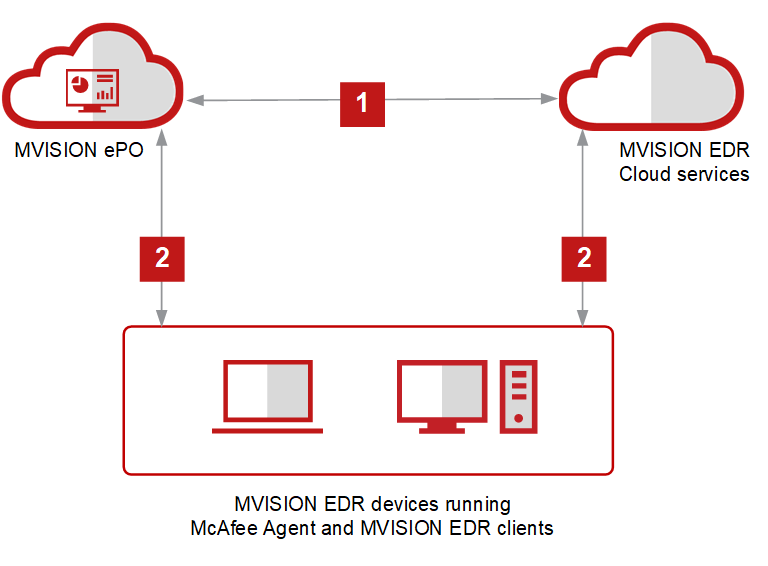
\includegraphics[width=0.85\textwidth]{misc/edr_centralized_model.png}
    \caption{Kiến trúc điển hình của một giải pháp EDR theo mô hình tập trung, trong đó toàn bộ thiết bị đầu cuối phải liên tục trao đổi dữ liệu với dịch vụ quản trị và phân tích trên nền tảng đám mây\protect\footnotemark.}
    \label{fig:edr-centralized}
\end{figure}
\footnotetext{Nguồn: \url{https://vietnetco.vn/solutions/soc-and-noc/edr}.}

Từ thực trạng đó, xu hướng nghiên cứu an toàn thông tin hiện đại tập trung vào việc dịch chuyển năng lực săn lùng và phát hiện mối đe dọa trực tiếp về phía máy trạm bằng trí tuệ nhân tạo biên (edge AI) và cơ chế phát hiện tại tác tử (agent-side). Hướng tiếp cận này cho phép tác tử tự hành phát hiện và phản ứng theo thời gian thực ngay tại điểm cuối mà không phụ thuộc vào kết nối mạng và hạ tầng đám mây. Để nhận diện các kỹ thuật tấn công đã biết với độ trễ thấp, các mẫu hành vi được chuẩn hóa theo ma trận MITRE ATT\&CK \cite{mitre_attack} và biểu diễn dưới định dạng luật phát hiện độc lập nền tảng như Sigma \cite{sigmahq}.

Xuất phát từ những phân tích trên, khóa luận lựa chọn nghiên cứu và xây dựng một giải pháp tác tử EDR tự hành chạy cục bộ trên hệ điều hành Windows, tích hợp trí tuệ nhân tạo biên và công nghệ đồ thị phả hệ tiến trình trong bộ nhớ nhằm phát hiện và ngăn chặn các kỹ thuật tấn công nâng cao theo thời gian thực, với độ trễ thấp, mức tiêu thụ tài nguyên tối ưu và khả năng phòng vệ độc lập kể cả khi thiết bị bị cô lập mạng.

\section{Mục tiêu đề tài}

\subsection{Mục tiêu tổng quát}

Mục tiêu tổng quát của khóa luận là nghiên cứu, thiết kế và xây dựng thành công một giải pháp tác tử phát hiện và phản ứng điểm cuối - EDR Agent tự hành trên hệ điều hành Windows, hoạt động cục bộ dưới dạng một dịch vụ hệ thống. Giải pháp tích hợp trí tuệ nhân tạo biên và công nghệ đồ thị phả hệ tiến trình trong bộ nhớ nhằm phát hiện và ngăn chặn lập tức các kỹ thuật tấn công bằng mã độc nâng cao, với độ trễ phản ứng thấp, tối ưu mức tiêu thụ tài nguyên máy trạm và bảo đảm khả năng phòng thủ ngay cả khi thiết bị bị cô lập mạng hoàn toàn.

\subsection{Mục tiêu cụ thể}

Để hiện thực hóa mục tiêu tổng quát, khóa luận xác định các mục tiêu cụ thể sau:

\begin{itemize}
    \item Xây dựng module thu thập dữ liệu giám sát ở mức nhân và cấu trúc hóa thành đồ thị quan hệ nhân quả trong bộ nhớ, bảo đảm thu thập đầy đủ bốn nhóm sự kiện hệ thống cốt lõi: Process, File, Registry, Network với mức tiêu thụ RAM ổn định.
    \item Phát triển động cơ tương quan hành vi dựa trên luật, có khả năng tự động hóa quy trình biên dịch luật phát hiện sang dạng thực thi hiệu năng cao, nhằm giảm thiểu đáng kể lượng sự kiện sạch cần xử lý và phát hiện các dòng lệnh độc hại phổ biến một cách nhanh chóng.
    \item Nghiên cứu, huấn luyện và tối ưu hóa động cơ trí tuệ nhân tạo biên có khả năng phân loại hành vi tiến trình, đồng thời tối ưu mô hình để suy diễn cục bộ theo thời gian thực với độ trễ thấp trên máy trạm.
    \item Xây dựng cơ chế phản ứng an toàn đa tầng, tổng hợp kết quả từ nhiều tầng phát hiện để đưa ra quyết định ngăn chặn tiến trình độc hại, và đóng gói toàn bộ các thành phần thành một phần mềm EDR Agent hoàn chỉnh, sẵn sàng vận hành trên Windows.
\end{itemize}

\section{Đối tượng và phạm vi nghiên cứu}

\subsection{Đối tượng nghiên cứu}

Đối tượng nghiên cứu của khóa luận bao gồm:

\begin{itemize}
    \item Kiến trúc nội tại của hệ điều hành Windows (Windows Internals) và các cơ chế giám sát mức nhân, trọng tâm là hạ tầng Event Tracing for Windows và Sysmon.
    \item Cấu trúc đồ thị nhân quả nguồn gốc (provenance graph) và các mô hình biểu diễn chuỗi hành vi của tiến trình.
    \item Các mô hình học máy và học sâu phục vụ phân loại hành vi và phát hiện bất thường tại điểm cuối.
    \item Định dạng luật phát hiện Sigma cho Windows và ma trận tri thức tấn công MITRE ATT\&CK.
    \item Nền tảng suy diễn mô hình ONNX Runtime C++ phục vụ triển khai trí tuệ nhân tạo cục bộ trên máy trạm.
\end{itemize}

\subsection{Phạm vi nghiên cứu}

Khóa luận giới hạn phạm vi nghiên cứu như sau:

\begin{itemize}
    \item \textbf{Hệ điều hành:} tập trung chuyên sâu vào hệ điều hành Microsoft Windows, bao gồm các phiên bản Windows 10, Windows 11 và Windows Server.
    \item \textbf{Phạm vi dữ liệu giám sát:} thu thập sự kiện qua ETW Kernel Providers (hoặc Sysmon) với bốn nhóm sự kiện cốt lõi: Process (tạo/hủy tiến trình, quan hệ tiến trình cha - con, tham số dòng lệnh), File (đọc, ghi, xóa/đổi tên hàng loạt), Registry (khóa tự khởi động, cơ chế duy trì hiện diện, thay đổi đặc quyền) và Network (kết nối outbound, truy vấn DNS).
    \item \textbf{Ứng dụng hướng đến:} tác tử EDR tự hành chạy dưới dạng Windows Service, bảo vệ máy trạm liên tục kể cả khi ngắt kết nối mạng.
\end{itemize}

\section{Phương pháp nghiên cứu}

\section{Cấu trúc khóa luận}
% Giới thiệu ngắn gọn nội dung từng chương.
